\chapter{Theory of attosecond transient absorption}
\label{atas_theory}

\section{Introduction}
\label{intro_atas_theory}

A common difficulty in working with extreme ultraviolet (XUV) light is the lack of efficient and broadband optics, especially beam splitters. Here, we introduce a method for generating two sources of XUV light by high harmonic generation using a phase grating.  This phase grating allows for precise and stable control of the phase delay between the two generate XUV beams.  This can be thought of as an inline interferometer, and it can have applications for XUV Fourier transform spectroscopy, as well as transient absorption spectroscopy \cite{diffuse}.

\section{Theory}
\label{theory_ts}

In order to generate two ostensibly identical XUV pulses, we take advantage of a diffractive optical element known as a beam splitting grating.   The idea is to introduce a periodic phase step in the beam, which will cause the beam to diffract into different orders.  The phase step is designed such that the +1 and -1 orders are most efficiently populated, with an efficiency of up to 81$\%$.  These will be used to generate spatially separated harmonics.

A key advantage to this method is that it allows for control of the relative phase between the two sources generating harmonics.  By translating the grating relative to the beam, the relative phase difference between the +1 and -1 orders goes from -2$\pi$ to 2$\pi$.  This can be seen in the phase of the electric field at the focus:



\begin{figure}
	\centering
	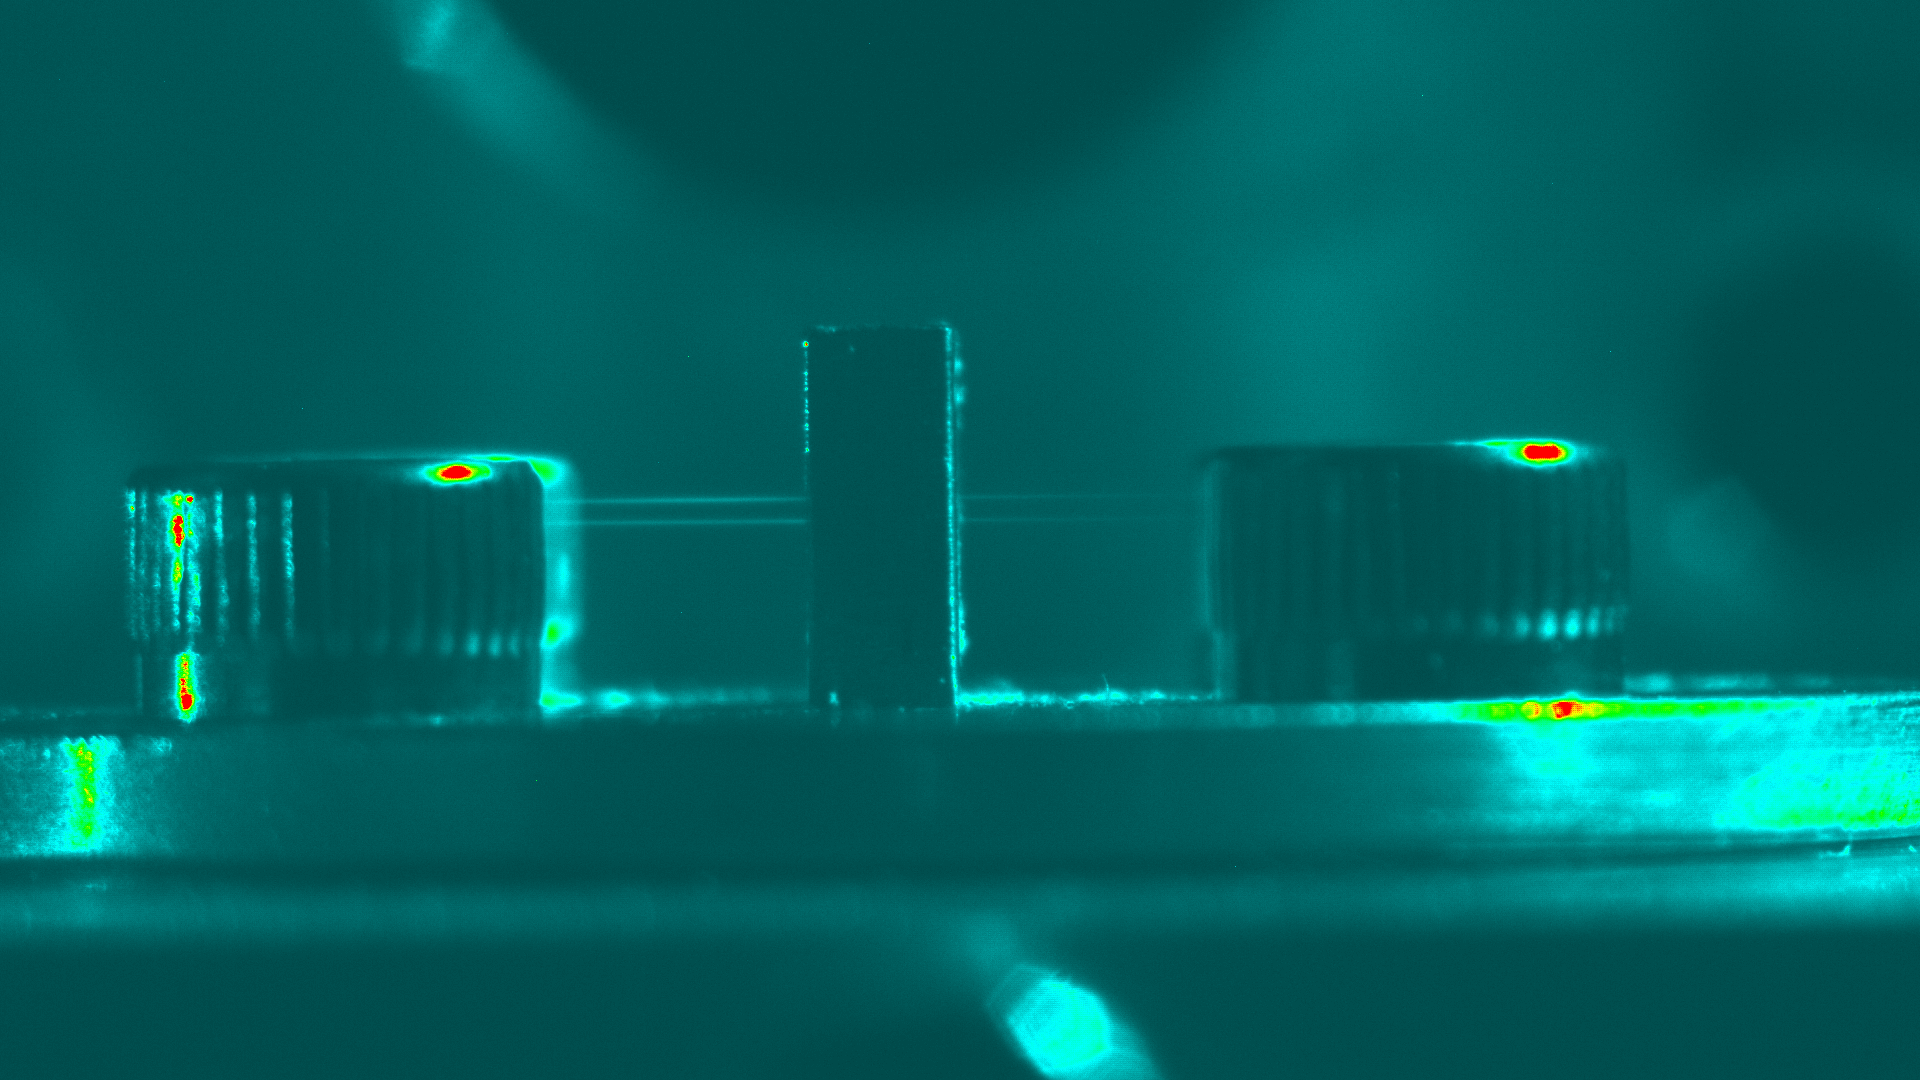
\includegraphics[width=0.9\textwidth]{figures/Two_source/ts_filament_gas_cell.png}
	\caption{Camera image of two sources generating a filament in a gas cell. Image was taken while chamber was vented and at ambient pressure.}
	\label{my_anita}
\end{figure}

\lipsum

\begin{figure}
	\centering
	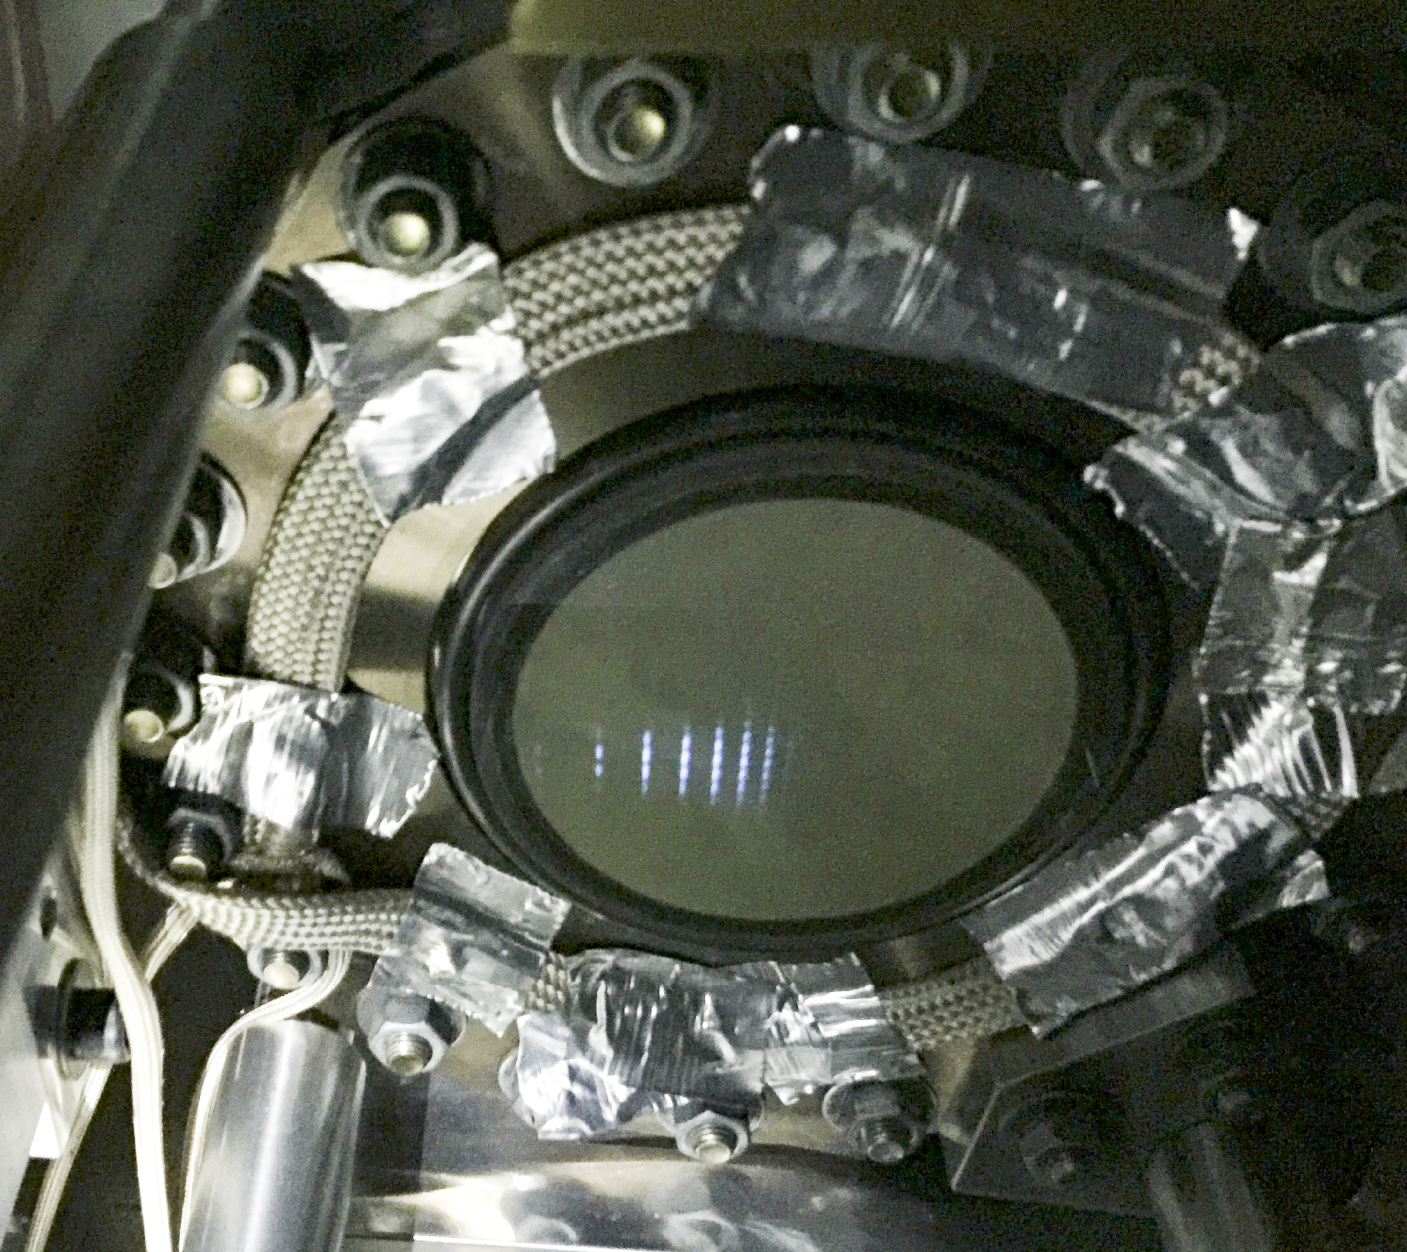
\includegraphics[width=0.9\textwidth]{figures/Two_source/MCP_ts_harmonics.png}
	\caption{Camera image of the output of the phosphor screen.  Harmonics are visible by eye.}
	\label{MCP_ts_harmonics}
\end{figure}

\lipsum

\begin{figure}
	\centering
	\includegraphics[width=0.9\textwidth]{figures/Two_source/dOD_dn.pdf}
	\caption{Camera image of two sources generating a filament in a gas cell. Image was taken while chamber was vented and at ambient pressure.}
	\label{my_anita}
\end{figure}

\lipsum